% REVISÃO DE LITERATURA--------------------------------------------------------

\chapter{FUNDAMENTAÇÃO TEÓRICA}
\label{chap:fundamentacaoTeorica}

Este capítulo tem como finalidade estabelecer a fundamentação teórica associada aos conceitos aqui abordados. Para tal, foram julgados como necessários os seguintes temas: Radiação Microondas (Seção 2.1), Magnetron (Seção 2.2), Fontes Ferro-Ressonantes (Seção 2.3), Funcionamento do forno microondas (Seção 2.4), Inversores ressonantes (Seção 2.5), Microcontroladores (Seção 2.6).

\section{RADIAÇÃO MICROONDAS}
\label{sec:radiacaoMicroondas}

A radiação microondas é uma forma da radiação eletromagnética com comprimento de ondas variando de 1 m a 1 mm, com frequências de 300 MHz até 300 GHz. O prefixo micro não tem intenção de sugerir a o comprimento de onda na ordem de grandeza de micrômetros. Este tipo de radiação viaja em linha de visada, não difratando em obstáculos terrestres como morros ou saliências, nem refletem na ionosfera, o que limita a comunicação ao horizonte visível, cerca de 64 km \cite{hitchcock}. Nas frequências mais altas da banda de microondas, os gases da atmosfera absorvem a radiação, limitando as comunicações nessa faixa em distâncias de cerca de 1km. Microondas são utilizadas de forma ampla nas aplicações tecnológicas modernas, tais como radares, redes \texttit{wi-fi}, tratamentos médicos, sistemas de prevenção de colisões, controles de garagem e fornos microondas. A figura abaixo compara a radiação microondas com as demais faixas de radiação eletromagnéticas

\begin{figure}[!htb]
    \centering
    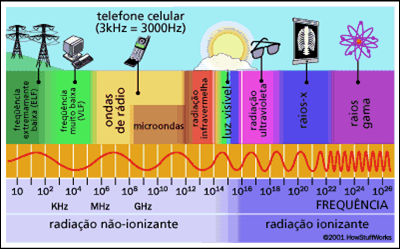
\includegraphics[width=0.75\textwidth]{./dados/figuras/figura_microondas}
    \caption{Comparação da radiação MO com as demais faixas de radiação eletromagnética}
    \fonte{\citeonline{trabalhoSeguro}}
    \label{fig:figura-mo}
\end{figure}

\section{MAGNETRON}
\label{sec:magnetron}

O magnetron consiste em um um tubo de vácuo de alta potência que gera radiação microondas através da interação de um fluxo de elétrons com um campo magnético. Os elétrons se movem entre uma série de cavidades de metal com aberturas chamadas de cavidades de ressonância. Um cátodo cilíndrico está no eixo principal, alguns milimetros distante de um ânodo circular. Dentro no ânodo, há diversas cavidades projetadas para ressonar em 2,45 GHz. Uma tensão da ordem de alguns kV é aplicada entre os eletrodos e um campo magnético é aplicado em paralelo ao eixo de forma que o campo elétrico e magnético fiquem perpendiculares entre si. Elétrons ejetados pelo cátodo aceleram radialmente no início devido ao campo elétrico mas começam a fazer trajetórias espirais devido a aceleração causada pelo campo magnético. Quando o campo magnético é forte demais, os elétrons não consegue chegar ao ânodo, e formam uma carga espacial giratória. As cavidades ressonantes do ânodo interagem com os elétrons, exercendo uma aceleração ou desaceleração. Finalmente, uma grande quantidade de elétrons oscila em volta do cátodo com frequências de microondas, que por sua vez gera oscilações auto-sustentáveis nas cavidades ressonantes, emitindo radiação microondas \cite{Vollmer}. A figura 2 mostra um diagrama do magnetron:

\begin{figure}[!htb]
    \centering
    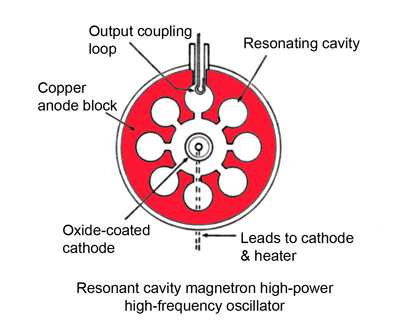
\includegraphics[width=0.75\textwidth]{./dados/figuras/magnetron}
    \caption{Diagrama de um Magnetron}
    \fonte{\citeonline{Vollmer}}
    \label{fig:figura-magnetron}
\end{figure}


\section{FONTES FERRO-RESSONANTES}
\label{sec:fontFerro}

Uma fonte ferro-ressonante é uma fonte baseada em transformador que usa características magnéticas não lineares e um circuito ressonante para providenciar uma tensão de saída estável sobre uma ampla faixa de tensões de entrada. Estas fontes são utilizadas em uma gama de aplicações que requerem tensões de saída constantes e especialmente utilizadas quando as tensões de entrada são instáveis devido à instabilidades das linhas de energia ou outros fatores, podendo absorver a maior parte dos transientes induzidos pela linha de transmissão. 

As fontes ferro-ressonantes são muito semelhantes a uma fonte incontrolável comum, exceto pelo fato da presença do transformador ferrorressonante, projetado especialmente para manter a tensão de saída constante em uma ampla faixa de tensões e correntes de entrada.  As principais desvantagens deste tipo de fonte são a sensibilidade a mudanças de frequência, a maior dissipação de calor em relação a transformadores comuns, a maior produção de ruído audível na ressonância e seu peso e tamanho em relação à fontes lineares \cite{PowerUk}. A figura 3 mostra um esquemático simplificado de uma fonte ferrorressonante, enquanto a figura 4 mostra uma fonte ferrorresonante em escala:


\begin{figure}[!htb]
    \centering
    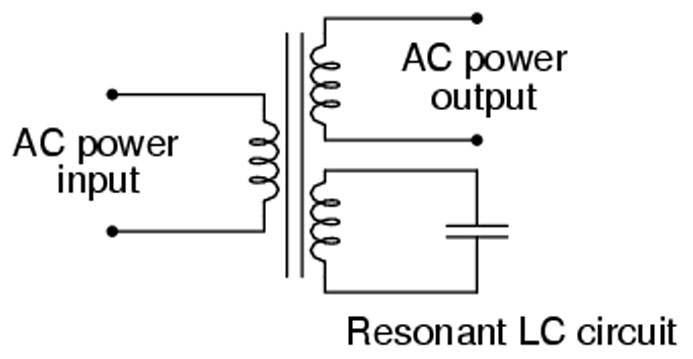
\includegraphics[width=0.6\textwidth]{./dados/figuras/font-ferro}
    \caption{Diagrama de uma fonte ferrorresonante}
    \fonte{\citeonline{PowerUk}}
    \label{fig:figura-fontferro}
\end{figure}

\pagebreak

\begin{figure}[!htb]
    \centering
    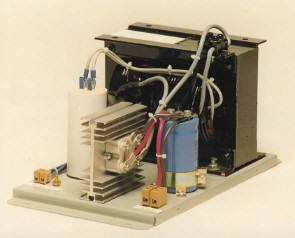
\includegraphics[width=0.4\textwidth]{./dados/figuras/font-ferro-real}
    \caption{Fonte ferrorresonante em escala}
    \fonte{\citeonline{PowerUk}}
    \label{fig:figura-fontferro}
\end{figure}



\section{FUNCIONAMENTO DO FORNO MICROONDAS}
\label{sec:funcMicro}

O forno microondas consiste em duas partes principais: o magnetron, o qual é alimentado por uma fonte com uma grande tensão de saída, e a câmara de cozimento, que é revestida por paredes metálicas e contém uma plataforma giratória para rotacionar o alimento. A medida que o magnetron gera radiação, as ondas eletromagnéticas chegam à câmara através de um guia de onda acoplado ao magnetron. Este guia geralmente é uma seção retangular de um tubo metálico. Uma vez que as MO chegam à câmara, elas são efetivamente refletidas pelas paredes metálicas. As ondas ressonam na cavidade e formam ondas estacionárias. Devido à frequência das ondas, cerca de 2,45 GHz, o comprimento de onda é da ordem das dimensões lineares da câmara. A figura abaixo mostra um diagrama de funcionamento de um forno convencional:

\begin{figure}[!htb]
    \centering
    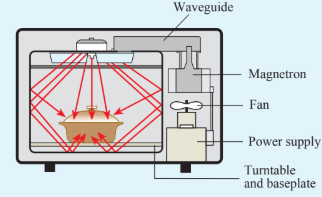
\includegraphics[width=0.6\textwidth]{./dados/figuras/microwave}
    \caption{Diagrama de funcionamento um forno microondas convencional}
    \fonte{\citeonline{Vollmer}}
    \label{fig:figura-fontferro}
\end{figure}

Num forno ideal, toda o alimento seria cozido de forma uniforme, porém, na prática os nós das ondas estacionárias geradas fazem que o alimento aqueça e algumas partes e permaneça frio em outras. A figura 6 mostra a distribuição de temperatura dentro de um forno microondas de dimensões  29 x 29 x 19 cm³, em um altura de cerca de 8 cm acima do fundo da cavidade. Um prato de vidro horizontal  com uma fina camada de água foi colocado 15 s em um microondas sem a plataforma giratória em potência máxima (cerca de 800 W). Com uma pequena quantidade de água presente, a imagem mostra o padrão de intensidade em uma câmara quase vazia. Nota-se uma existência pronunciada de modos de ressonância horizontais, o que geraria um aquecimento não uniforme. Esta não uniformidade é a principal razão para a existência da plataforma giratória, que levaria o alimento a diferentes nós quentes e frios \cite{Vollmer}. No entanto, mesmo com a plataforma o alimento ainda é cozido de forma não uniforme, devido à complexa interação entre as MO e os alimentos e as diferentes interações que cada parte do alimento tem com cada um dos nós e antinós.

\begin{figure}[!htb]
    \centering
    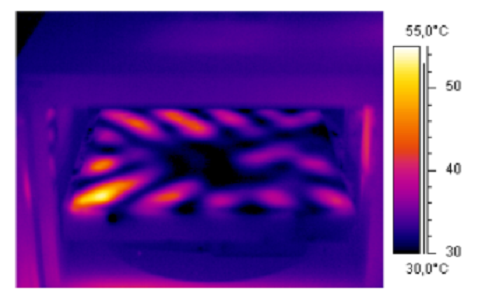
\includegraphics[width=0.6\textwidth]{./dados/figuras/micronodes}
    \caption{Visualização da estrutura dos modos de propagação horizontais em um forno microondas utilizando imagens termais infravermelhas. Um prato de vidro com uma fina camada de água foi colocado de uma altura de 8 cm e aquecido por 15 s em uma potência de 800 W.}
    \fonte{\citeonline{Vollmer}}
    \label{fig:figura-fontferro}
\end{figure}


\section{INVERSORES RESSONANTES}
\label{sec:inverter}

Inversores ressonantes são um tipo de inversor baseados em oscilações ressonantes de corrente.  Inversores ressonantes série são colocados em série com a carga para formar um circuito sub-amortecido. A corrente através destes dispositivos de chaveamento chega a zero devido a natureza do circuito. Se o dispositivo for um tiristor, diz-se que o dispositivo é auto-comutado. 
Este tipo de inversor produz uma forma onda aproximadamente senoidal de frequências que podem variar de 20 kHz até 100 MHz e é comumente usados em aplicações que necessitam de tensão constante, como lâmpadas fluorescentes, geradores ultra sônicos ou aquecimento por indução. Devido a alta frequência de chaveamento, os componentes do inversor ressonantes tem tamanho reduzido \cite{Rashid}.

\begin{figure}[!htb]
    \centering
    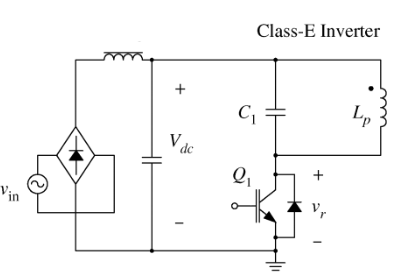
\includegraphics[width=0.6\textwidth]{./dados/figuras/inverter}
    \caption{Inversor ressonante classe E}
    \fonte{\citeonline{Woo}}
    \label{fig:figura-fontferro}
\end{figure}



\section{MICROCONTROLADORES}
\label{sec:micro}

Um microcontrolador, ou UC (acrônimo para   $\mu$-controlador) é um pequeno computador em um único circuito integrado. Um microcontrolador pode ter uma ou mais CPUs, isto é núcleos de processamento, juntamente com uma memória e periféricos de entrada e saída programáveis. Memória na forma de \texit{flash} ou ROM é inclusa no \texit{chip}, em conjunto com uma pequena quantidade de memória RAM. Microcontroladores são projetados para aplicações embarcadas, em contraste com os microprocessadores utilizados nos computadores pessoais. Geralmente os UC são aplicados em produtos ou dispositivos controlados automaticamente, tais como sistemas de controle para motores ou controles remotos. Por terem tamanhos e custo reduzidos em relação a um projeto que utiliza um microprocessador, memória e dispositivos de I/O separadamente, os UC são economicamente vantajosos para fazer o controle de um dispositivo ou processo.

\pagebreak 

\begin{figure}[t]
    \centering
    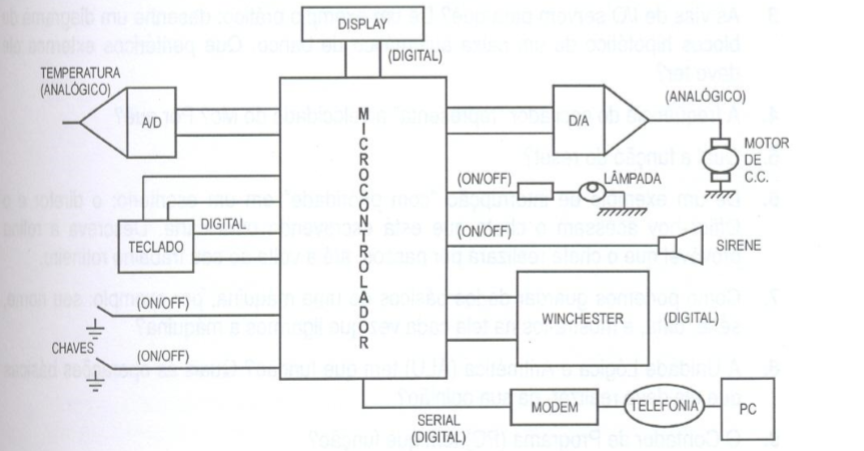
\includegraphics[width=0.9\textwidth]{./dados/figuras/micro}
    \caption{Ilustração hipotética de um microcontrolador e seus periféricos}
    \fonte{\citeonline{Nicolosi}}
    \label{fig:figura-mvc}
\end{figure}

\null
\vfill


            
